% Manuscrito de papa-vision — versión en español, con formato tipo Nature Scientific Reports.
% Autónomo: usa sólo paquetes LaTeX estándar para compilar con pdflatex + bibtex.
% Los números y las tablas se generan automáticamente a partir de las métricas
% versionadas (scripts/make_paper_tables.py) y se incorporan con \input más abajo.
\documentclass[10pt]{article}

\usepackage[utf8]{inputenc}
\usepackage[T1]{fontenc}
\usepackage[spanish,es-noshorthands]{babel}
\usepackage{lmodern}
\usepackage[a4paper,margin=2.2cm]{geometry}
\usepackage{graphicx}
\usepackage{amsmath}
\usepackage{booktabs}
\usepackage{caption}
\usepackage{authblk}
\usepackage{xcolor}
\usepackage[colorlinks=true,linkcolor=blue,citecolor=blue,urlcolor=blue]{hyperref}
\usepackage{titlesec}

\graphicspath{{figures/}}
\captionsetup{font=small,labelfont=bf}
\titleformat{\section}{\large\bfseries\color{black!85}}{\thesection}{0.6em}{}
\titleformat{\subsection}{\normalsize\bfseries}{\thesubsection}{0.5em}{}

% Carga PRIMERO los macros de métricas auto-generados (\newcommand reales);
% los \providecommand de respaldo de abajo sólo rellenan lo que falte, de modo
% que el documento también compila por sí solo antes de generar las métricas.
\IfFileExists{results_macros.tex}{% Auto-generated by scripts/make_paper_tables.py — do not edit.
\newcommand{\accCustom}{97.3}
\newcommand{\foneCustom}{96.7}
\newcommand{\eceCustom}{0.123}
\newcommand{\paramsCustom}{328{,}587}
\newcommand{\trainparamsCustom}{328{,}587}
\newcommand{\accMobilenet}{94.9}
\newcommand{\foneMobilenet}{91.6}
\newcommand{\eceMobilenet}{0.134}
\newcommand{\paramsMobilenet}{2{,}227{,}715}
\newcommand{\trainparamsMobilenet}{3{,}843}
\newcommand{\accResnet}{91.7}
\newcommand{\foneResnet}{86.5}
\newcommand{\eceResnet}{0.171}
\newcommand{\paramsResnet}{11{,}178{,}051}
\newcommand{\trainparamsResnet}{1{,}539}
\newcommand{\accEfficientnet}{94.9}
\newcommand{\foneEfficientnet}{91.7}
\newcommand{\eceEfficientnet}{0.157}
\newcommand{\paramsEfficientnet}{4{,}011{,}391}
\newcommand{\trainparamsEfficientnet}{3{,}843}
\newcommand{\ntrain}{1506}
\newcommand{\nval}{323}
\newcommand{\ntest}{323}
\newcommand{\ntotal}{2152}
\newcommand{\nseeds}{3}
\newcommand{\bestmodel}{Custom CNN (scratch)}
\newcommand{\bestfone}{96.7}
\newcommand{\bestfoneCIlo}{93.6}
\newcommand{\bestfoneCIhi}{99.5}
\newcommand{\bestaccCIlo}{96.6}
\newcommand{\bestaccCIhi}{99.4}
\newcommand{\traincustom}{328{,}587}
\newcommand{\trainheadmin}{1{,}539}
\newcommand{\trainheadmax}{3{,}843}
\newcommand{\hpotrials}{10}
\newcommand{\hpobestfone}{96.9}
\newcommand{\hpolr}{0.001}
\newcommand{\hpowd}{1e-05}
\newcommand{\hpowidth}{24}
\newcommand{\hpodropout}{0.3}
\newcommand{\hpoaug}{0.5}
\newcommand{\besttransfer}{EfficientNet-B0}
\newcommand{\besttransferfone}{91.7}
\newcommand{\paramratiomin}{7}
\newcommand{\paramratiomax}{34}
\newcommand{\mcnemarbestp}{0.0169}
\newcommand{\mcnemarbestverdict}{a significant difference}
}{}

% --- Respaldos para que el documento compile incluso sin métricas generadas. ---
\providecommand{\accCustom}{--}\providecommand{\foneCustom}{--}\providecommand{\eceCustom}{--}
\providecommand{\paramsCustom}{--}\providecommand{\trainparamsCustom}{--}
\providecommand{\accMobilenet}{--}\providecommand{\foneMobilenet}{--}\providecommand{\eceMobilenet}{--}\providecommand{\paramsMobilenet}{--}\providecommand{\trainparamsMobilenet}{--}
\providecommand{\accResnet}{--}\providecommand{\foneResnet}{--}\providecommand{\eceResnet}{--}\providecommand{\paramsResnet}{--}\providecommand{\trainparamsResnet}{--}
\providecommand{\accEfficientnet}{--}\providecommand{\foneEfficientnet}{--}\providecommand{\eceEfficientnet}{--}\providecommand{\paramsEfficientnet}{--}\providecommand{\trainparamsEfficientnet}{--}
\providecommand{\ntrain}{--}\providecommand{\nval}{--}\providecommand{\ntest}{--}\providecommand{\ntotal}{--}\providecommand{\nseeds}{--}
\providecommand{\bestmodel}{--}\providecommand{\bestfone}{--}\providecommand{\besttransfer}{el mejor modelo por transferencia}\providecommand{\besttransferfone}{--}
\providecommand{\paramratiomin}{--}\providecommand{\paramratiomax}{--}
\providecommand{\bestfoneCIlo}{--}\providecommand{\bestfoneCIhi}{--}\providecommand{\bestaccCIlo}{--}\providecommand{\bestaccCIhi}{--}
\providecommand{\traincustom}{--}\providecommand{\trainheadmin}{--}\providecommand{\trainheadmax}{--}
\providecommand{\hpotrials}{--}\providecommand{\hpobestfone}{--}\providecommand{\hpolr}{--}\providecommand{\hpowd}{--}\providecommand{\hpowidth}{--}\providecommand{\hpodropout}{--}\providecommand{\hpoaug}{--}
\providecommand{\mcnemarbestp}{--}\providecommand{\mcnemarbestverdict}{--}

\title{\vspace{-1.0cm}\bfseries Redes neuronales convolucionales ligeras para el
diagnóstico de enfermedades en hojas de papa con hardware de consumo: un estudio de
entrenamiento desde cero frente al aprendizaje por transferencia con interpretabilidad
mediante Grad-CAM}

\author[1]{Niels Pacheco}
\affil[1]{Programa de Maestría en Inteligencia Artificial, MIA-07 Redes Neuronales
y Aprendizaje Profundo (Sección C). \texttt{nielspacheco1997@gmail.com}}

\date{Junio de 2026}

\begin{document}
\maketitle

\begin{abstract}
\noindent
Las enfermedades foliares como el tizón temprano (\textit{Alternaria solani}) y el
tizón tardío (\textit{Phytophthora infestans}) amenazan a la papa
(\textit{Solanum tuberosum}), el cultivo básico domesticado en los Andes peruanos y
el tercer alimento más importante del mundo. Las redes neuronales convolucionales
(CNN) pueden reconocer estas enfermedades a partir de fotografías de hojas, pero la
mayoría de los sistemas reportados dependen de grandes redes preentrenadas y de
unidades de procesamiento gráfico (GPU) que no están al alcance de los pequeños
agricultores que más se beneficiarían. Nos preguntamos si una CNN compacta entrenada
\emph{desde cero} en hardware de consumo (una laptop con CPU/Apple Silicon, sin GPU)
puede rivalizar con los modelos de aprendizaje por transferencia preentrenados en
ImageNet para la clasificación de hojas de papa en tres clases (sana, tizón temprano,
tizón tardío). Sobre el subconjunto de papa de PlantVillage ($\ntotal$ imágenes)
comparamos una CNN propia de $\paramsCustom$ parámetros frente a MobileNetV2,
ResNet-18 y EfficientNet-B0 con redes base de ImageNet congeladas y cabezales
ajustados, evaluando cada modelo sobre $\nseeds$ semillas aleatorias, reportando
desviaciones estándar entre semillas e intervalos de confianza no paramétricos por
\emph{bootstrap}, con pruebas de significancia de McNemar y análisis de calibración.
Sorprendentemente, la CNN propia entrenada desde cero alcanza $\foneCustom\%$ de F1
macro, \emph{superando} al mejor modelo por transferencia
(\besttransfer{}, $\besttransferfone\%$); las pruebas pareadas de McNemar confirman
que supera significativamente a los tres modelos por transferencia de red base
congelada ($p<0.05$) usando del orden de $\paramratiomin$--$\paramratiomax\times$
menos parámetros. El resultado indica que, bajo un presupuesto de cómputo igualmente
bajo, aprender de extremo a extremo características compactas y específicas del dominio
supera a reutilizar características congeladas de ImageNet. No obstante, los mapas de
saliencia de Grad-CAM indican que todos los modelos atienden en parte al fondo de la
imagen y no a las lesiones de la hoja, en concordancia cualitativa con el bien
documentado sesgo de fondo de PlantVillage, lo que matiza las exactitudes optimistas.
Publicamos una canalización totalmente reproducible---entorno fijado, semillas fijas,
experimentos dirigidos por configuración y una construcción de este manuscrito con un
solo comando---para apoyar una investigación de enfermedades vegetales honesta y
accesible en hardware.
\end{abstract}

\section{Introducción}
La papa es el tercer cultivo alimentario más importante para el consumo humano en el
mundo y fue domesticada por primera vez hace más de siete mil años en las tierras
altas de lo que hoy es Perú y Bolivia~\cite{fao2008potato}. Su productividad está
crónicamente amenazada por enfermedades foliares. El tizón tardío, causado por el
oomiceto \textit{Phytophthora infestans}, desencadenó la hambruna irlandesa del siglo
XIX y sigue siendo hoy la enfermedad más destructiva de la papa, capaz de arrasar un
campo entero en cuestión de días~\cite{fry2008phytophthora}. El tizón temprano,
causado por el hongo \textit{Alternaria solani}, también está muy extendido. La
identificación temprana y precisa de estas enfermedades a partir de los síntomas
foliares permite una intervención oportuna, pero el diagnóstico experto es escaso en
las comunidades rurales andinas donde se concentra el cultivo de la papa.

El aprendizaje profundo ofrece una vía hacia un diagnóstico democratizado. Desde que
se demostró que las CNN pueden clasificar imágenes de enfermedades vegetales con alta
exactitud~\cite{mohanty2016using,ferentinos2018deep}, una amplia literatura ha
aplicado redes preentrenadas cada vez más grandes al problema. Sin embargo, dos
preocupaciones prácticas están poco examinadas. Primero, la mayoría de los sistemas
asume acceso a GPU y a grandes redes preentrenadas, un supuesto reñido con los
entornos de recursos limitados donde la tecnología es más necesaria. Segundo, las
exactitudes destacadas del campo se reportan con frecuencia sin intervalos de
confianza, sin análisis de calibración y sin verificación alguna de que el modelo
atienda a la enfermedad y no a correlaciones espurias del conjunto de datos.

Este trabajo aborda ambas preocupaciones mediante un estudio enfocado y reproducible.
Planteamos una sola pregunta: \emph{¿qué tan cerca puede llegar una CNN pequeña
entrenada desde cero en una laptop sin GPU al aprendizaje por transferencia
preentrenado en ImageNet para la clasificación de enfermedades en hojas de papa?}
Nuestras contribuciones son:
\begin{enumerate}
  \item Una CNN propia compacta ($\paramsCustom$ parámetros) que se entrena de
  extremo a extremo en hardware CPU o Apple Silicon, comparada directamente con
  modelos de aprendizaje por transferencia (MobileNetV2, ResNet-18 y EfficientNet-B0
  con redes base de ImageNet congeladas y cabezales de clasificación ajustados).
  \item Una evaluación estadísticamente rigurosa---corridas con múltiples semillas y
  desviaciones estándar entre semillas, intervalos de confianza por \emph{bootstrap}
  al 95\% por corrida, y la prueba pareada de McNemar sobre un conjunto de prueba
  compartido~\cite{dietterich1998mcnemar}---en lugar de un único número de exactitud.
  \item Un análisis de calibración (error de calibración esperado y diagramas de
  fiabilidad)~\cite{guo2017calibration}, rara vez reportado en el trabajo de
  enfermedades vegetales.
  \item Un estudio de interpretabilidad con Grad-CAM~\cite{selvaraju2017gradcam} que
  sondea el documentado sesgo de fondo de PlantVillage~\cite{noyan2022uncovering}, con
  una discusión honesta de la brecha entre el rendimiento de laboratorio y el de campo.
  \item Una publicación de código abierto totalmente reproducible (dependencias
  fijadas, semillas fijas, corridas dirigidas por configuración, generación
  automatizada de figuras y del manuscrito).
\end{enumerate}

\section{Trabajo relacionado}
\textbf{Clasificación de enfermedades vegetales.} Mohanty et al.~\cite{mohanty2016using}
entrenaron AlexNet y GoogLeNet sobre el conjunto PlantVillage y reportaron exactitudes
superiores al 99\% bajo evaluación dentro del mismo conjunto, estableciendo el punto de
referencia que sigue gran parte del trabajo posterior.
Ferentinos~\cite{ferentinos2018deep} extendió el enfoque a docenas de combinaciones
cultivo-enfermedad. De manera crucial, Barbedo~\cite{barbedo2018impact} mostró que
tales exactitudes se degradan abruptamente cuando los modelos se evalúan con imágenes
recolectadas en condiciones distintas, atribuyendo la caída a la limitada variedad del
conjunto de datos y a las señales del fondo, y Noyan~\cite{noyan2022uncovering}
demostró explícitamente que un clasificador puede recuperar las etiquetas de
PlantVillage a partir \emph{únicamente del fondo}. Tomamos en serio esta crítica y la
ponemos a prueba directamente con Grad-CAM.

\textbf{Arquitecturas eficientes y de transferencia.} Las conexiones residuales
permitieron entrenar redes muy profundas~\cite{he2016resnet};
MobileNetV2~\cite{sandler2018mobilenetv2} y EfficientNet~\cite{tan2019efficientnet}
optimizaron después el compromiso entre exactitud y número de parámetros para el
despliegue con recursos limitados. El aprendizaje por transferencia desde
ImageNet~\cite{russakovsky2015imagenet} es la receta por defecto para conjuntos de
datos pequeños. Nuestro estudio usa estas redes base como líneas base fuertes, pero se
pregunta qué es recuperable \emph{sin} sus pesos preentrenados.

\textbf{Interpretabilidad.} Grad-CAM~\cite{selvaraju2017gradcam} produce mapas de
saliencia discriminativos por clase ponderando las activaciones convolucionales con los
gradientes del puntaje de clase, y se ha convertido en una herramienta estándar para
verificar que la evidencia de un modelo sea plausible. La usamos no para confirmar el
éxito, sino para exponer un modo de fallo.

\section{Métodos}
\subsection{Conjunto de datos}
Usamos el subconjunto de papa de PlantVillage~\cite{hughes2015plantvillage}, que
comprende $\ntotal$ imágenes RGB de hojas en tres clases---sana, tizón temprano y
tizón tardío---fotografiadas en condiciones controladas de laboratorio
(Fig.~\ref{fig:samples}). Las clases están desbalanceadas (la clase sana es la más
pequeña). Particionamos los datos una sola vez en conjuntos de entrenamiento,
validación y prueba de aproximadamente 70/15/15\%, estratificados por clase, usando una
semilla de partición fija de modo que \emph{todos} los modelos se entrenan y evalúan en
particiones idénticas; esto da $\ntrain$ imágenes de entrenamiento, $\nval$ de
validación y $\ntest$ de prueba. Mantener la partición fija es lo que hace válida la
prueba pareada de McNemar entre modelos.

\begin{figure}[t]
\centering
\IfFileExists{figures/dataset_samples.png}{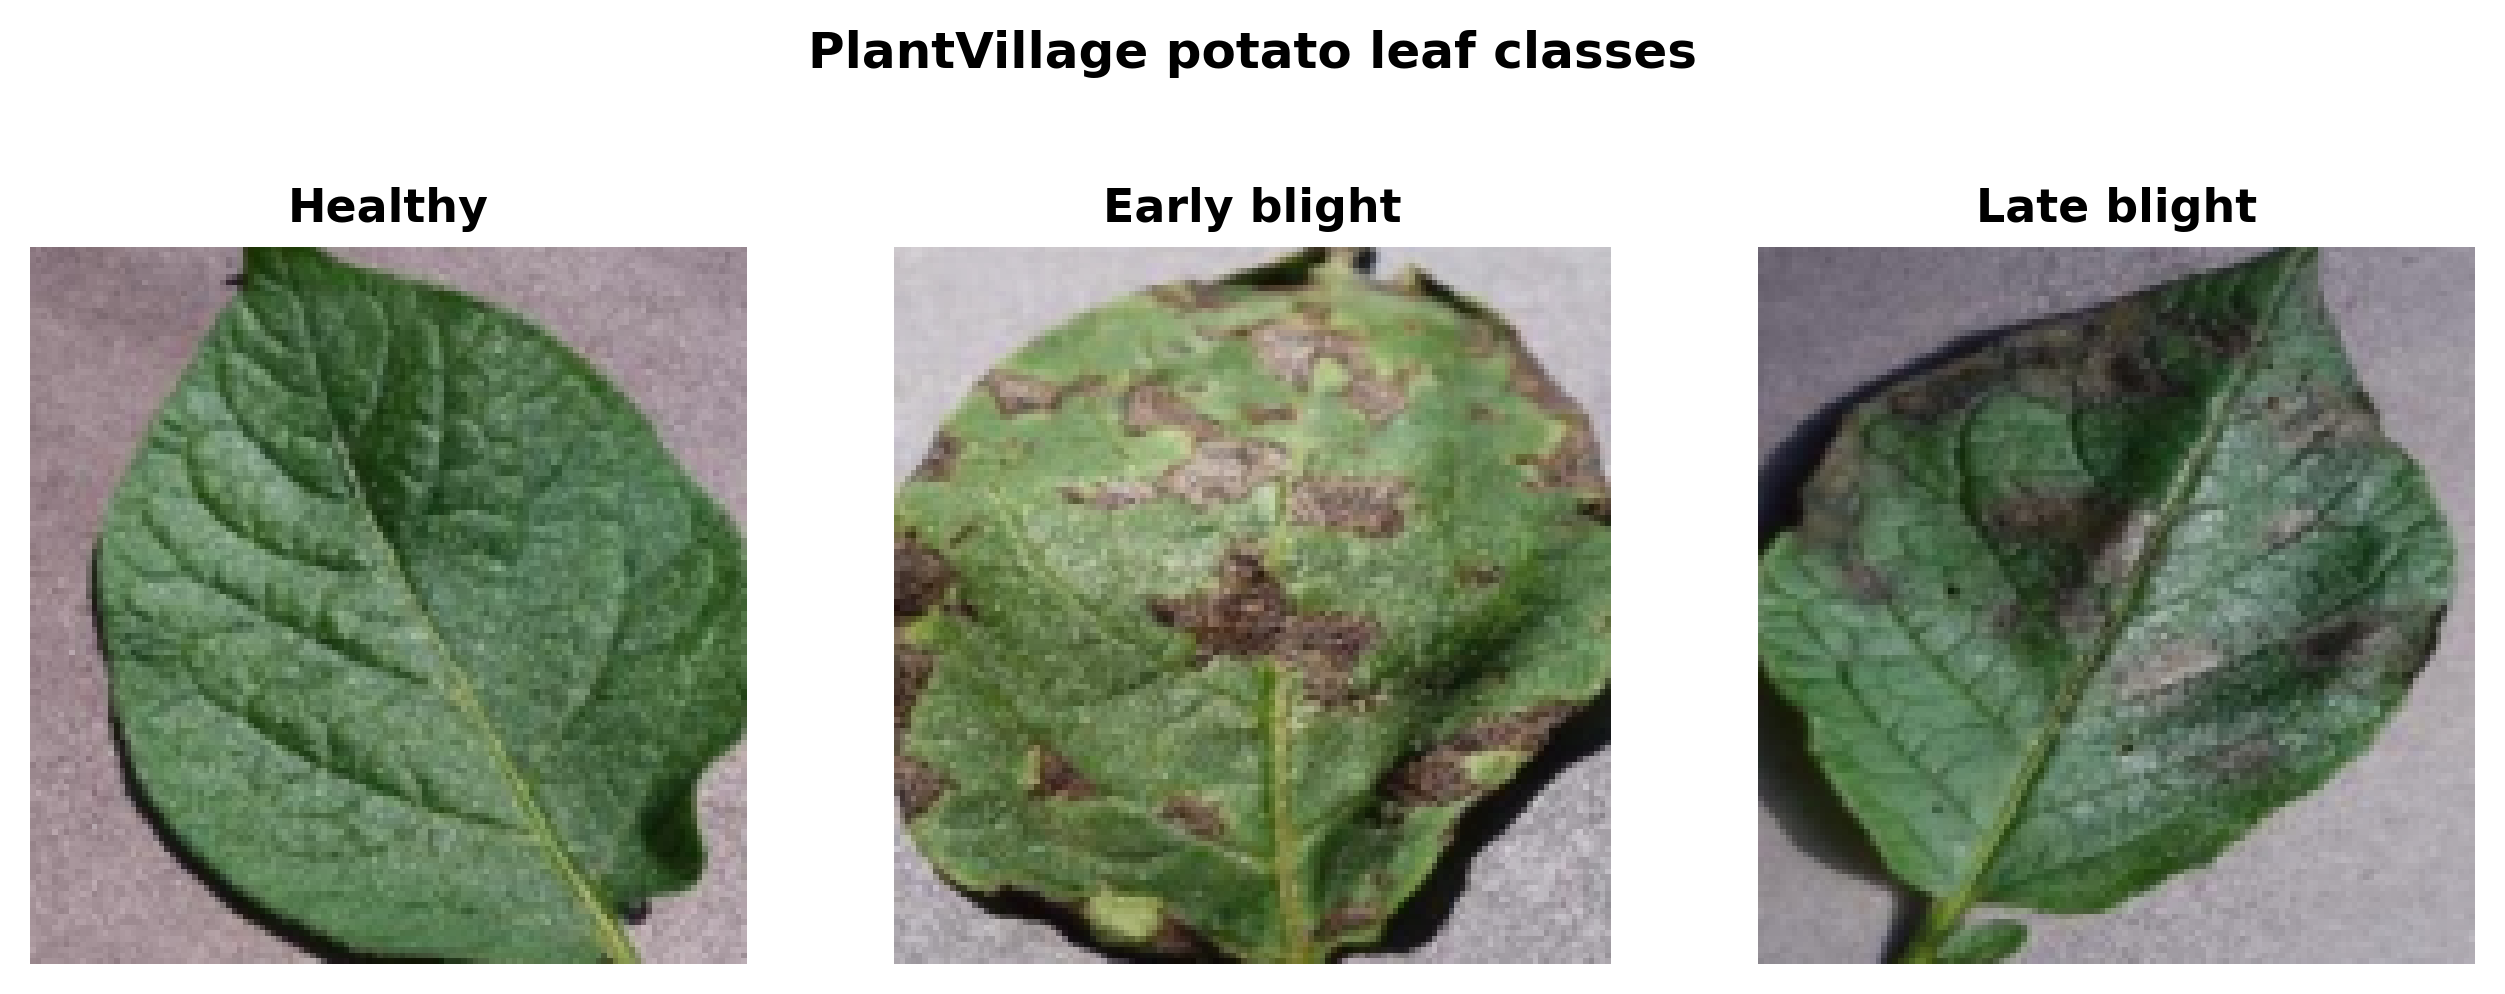
\includegraphics[width=0.85\linewidth]{dataset_samples.png}}{\fbox{\parbox{0.6\linewidth}{\centering\vspace{1cm}[dataset\_samples.png]\vspace{1cm}}}}
\caption{Imágenes representativas de hojas de papa de cada clase, tomadas del conjunto
de prueba reservado. Las imágenes de PlantVillage se capturan sobre fondos bastante
uniformes---una propiedad que, como mostramos, los modelos pueden explotar.}
\label{fig:samples}
\end{figure}

\subsection{Preprocesamiento y aumentación}
Las imágenes se redimensionan y recortan al centro a $128\times128$ píxeles y se
normalizan con las estadísticas de canal de ImageNet (aplicadas de manera uniforme a
todos los modelos para que sólo difieran la arquitectura y los pesos). Durante el
entrenamiento aplicamos recorte aleatorio redimensionado, volteo horizontal, pequeñas
rotaciones y variación de color (\emph{color jitter}), con una intensidad de
aumentación seleccionada por la búsqueda de hiperparámetros.

\subsection{Modelos}
La \textbf{CNN propia} es una red de cuatro bloques construida desde cero: cada bloque
aplica dos convoluciones de $3\times3$ con normalización por
lotes~\cite{ioffe2015batchnorm} y activaciones ReLU seguidas de \emph{max pooling}, con
anchos de canal que crecen y luego se estabilizan para mantener el modelo compacto
($\paramsCustom$ parámetros). Una capa de \emph{global average pooling} alimenta a un
clasificador lineal regularizado con \emph{dropout}~\cite{srivastava2014dropout}. Las
tres \textbf{líneas base por transferencia}---MobileNetV2~\cite{sandler2018mobilenetv2},
ResNet-18~\cite{he2016resnet} y EfficientNet-B0~\cite{tan2019efficientnet}---se
inicializan con pesos preentrenados en ImageNet; congelamos cada red base y entrenamos
sólo un nuevo cabezal de clasificación, la receta estándar de transferencia con pocos
datos.

\subsection{Entrenamiento}
Todos los modelos se entrenan con el optimizador AdamW~\cite{loshchilov2019adamw,kingma2014adam},
una planificación coseno de la tasa de aprendizaje, entropía cruzada ponderada por
clase con suavizado de etiquetas~\cite{szegedy2016labelsmoothing} para contrarrestar el
desbalance de clases, y parada temprana sobre el F1 macro de validación. Los
hiperparámetros de la CNN propia se seleccionaron mediante una búsqueda aleatoria con
semilla de $\hpotrials$ configuraciones sobre tasa de aprendizaje, decaimiento de
pesos, ancho de la red, \emph{dropout} e intensidad de aumentación, optimizando
únicamente el F1 macro de validación (el conjunto de prueba nunca se consulta durante
la selección del modelo). La búsqueda seleccionó una tasa de aprendizaje de $\hpolr$,
decaimiento de pesos $\hpowd$, ancho $\hpowidth$, \emph{dropout} $\hpodropout$ e
intensidad de aumentación $\hpoaug$. Todos los experimentos corren en una laptop Apple
Silicon usando el \emph{backend} Metal (MPS) de PyTorch~\cite{paszke2019pytorch}; no se
usa GPU.

\subsection{Evaluación y estadística}
Para cada modelo reportamos exactitud y F1 promediado por macro (robusto al desbalance
de clases), cada uno como media y desviación estándar sobre $\nseeds$ semillas
aleatorias (Cuadro~\ref{tab:results}, Fig.~\ref{fig:comparison}). Para cuantificar la
incertidumbre de muestreo dentro del conjunto de prueba, además calculamos intervalos
de confianza no paramétricos al 95\% mediante remuestreo \emph{bootstrap} del conjunto
de prueba para cada corrida; estos se publican con las métricas por corrida y los
intervalos del mejor modelo se citan en los Resultados. Comparamos los modelos por
pares sobre su conjunto de prueba compartido con la prueba de
McNemar~\cite{dietterich1998mcnemar}, usando la forma binomial exacta cuando el número
de predicciones discordantes es pequeño. Evaluamos la calibración con el error de
calibración esperado (ECE) y diagramas de fiabilidad~\cite{guo2017calibration}. Por
último, calculamos mapas de saliencia de Grad-CAM~\cite{selvaraju2017gradcam} para
inspeccionar qué regiones de la imagen impulsan cada predicción.

\section{Resultados}
\IfFileExists{tables_es.tex}{% Versión en español de las tablas (números idénticos a tables.tex, auto-generado).
\begin{table}[t]
\centering
\caption{Rendimiento en el conjunto de prueba sobre la partición reservada de hojas de papa ($n=323$ imágenes), reportado como media\,$\pm$\,desviación estándar sobre 3 semillas aleatorias. La exactitud y el F1 macro están en porcentaje; ECE es el error de calibración esperado (menor es mejor). Params = parámetros totales.}
\label{tab:results}
\begin{tabular}{lrccc}
\hline
Modelo & Params & Exactitud (\%) & F1 macro (\%) & ECE \\
\hline
CNN propia (desde cero) & 328{,}587 & 97.3\,$\pm$\,2.3 & \textbf{96.7\,$\pm$\,2.1} & 0.123 \\
MobileNetV2 & 2{,}227{,}715 & 94.9\,$\pm$\,0.8 & {91.6\,$\pm$\,1.2} & 0.134 \\
ResNet-18 & 11{,}178{,}051 & 91.7\,$\pm$\,1.5 & {86.5\,$\pm$\,2.1} & 0.171 \\
EfficientNet-B0 & 4{,}011{,}391 & 94.9\,$\pm$\,0.5 & {91.7\,$\pm$\,1.4} & 0.157 \\
\hline
\end{tabular}
\end{table}

\begin{table}[t]
\centering
\caption{Métricas de prueba por clase para el mejor modelo (CNN propia (desde cero), semilla representativa). El soporte es el número de imágenes de prueba por clase.}
\label{tab:perclass}
\begin{tabular}{lcccc}
\hline
Clase & Precisión & Sensibilidad & F1 & Soporte \\
\hline
Sana & 0.917 & 0.957 & 0.936 & 23 \\
Tizón temprano & 0.980 & 1.000 & 0.990 & 150 \\
Tizón tardío & 0.993 & 0.967 & 0.980 & 150 \\
\hline
\end{tabular}
\end{table}
}{}

\subsection{Desempeño de clasificación}
El Cuadro~\ref{tab:results} resume el desempeño de prueba. Los cuatro modelos
clasifican las tres condiciones de la papa con exactitud, reflejando la naturaleza
relativamente limpia y controlada en laboratorio de PlantVillage. El resultado
destacado, sin embargo, es que la CNN propia entrenada desde cero no sólo es
competitiva sino la \emph{mejor}: con apenas $\paramsCustom$ parámetros alcanza
$\foneCustom\%$ de F1 macro, por delante del mejor modelo por transferencia
(\besttransfer{}, $\besttransferfone\%$) y muy por delante de ResNet-18
(Fig.~\ref{fig:comparison}). Las pruebas pareadas de McNemar sobre el conjunto de
prueba compartido (semilla 0) encuentran que la CNN propia es significativamente mejor
que cada línea base de red base congelada ($p=\mcnemarbestp$ frente a \besttransfer{},
y menor frente a las demás; véase \texttt{summary.json} en el repositorio). Un
\emph{bootstrap} no paramétrico sobre ese conjunto de prueba sitúa el F1 macro de la
CNN propia en $[\bestfoneCIlo, \bestfoneCIhi]\%$ (IC al 95\%) y su exactitud en
$[\bestaccCIlo, \bestaccCIhi]\%$. La prueba de significancia se calcula sobre las
predicciones de una sola semilla, pero el orden no es específico de la semilla: en las
tres semillas, el F1 macro medio de la CNN propia ($\foneCustom\%$) supera la media de
cada línea base. La interpretación es que, cuando sólo puede entrenarse un pequeño
cabezal de clasificación sobre una red base de ImageNet congelada, esas redes base
aportan características genéricas mal ajustadas a la patología foliar, mientras que la
CNN compacta---entrenada de extremo a extremo---aprende características específicas de
la tarea. Las curvas de F1 macro de validación (Fig.~\ref{fig:curves}) muestran que
todos los modelos alcanzan una meseta alta dentro del presupuesto de entrenamiento.

\begin{figure}[t]
\centering
\IfFileExists{figures/model_comparison.png}{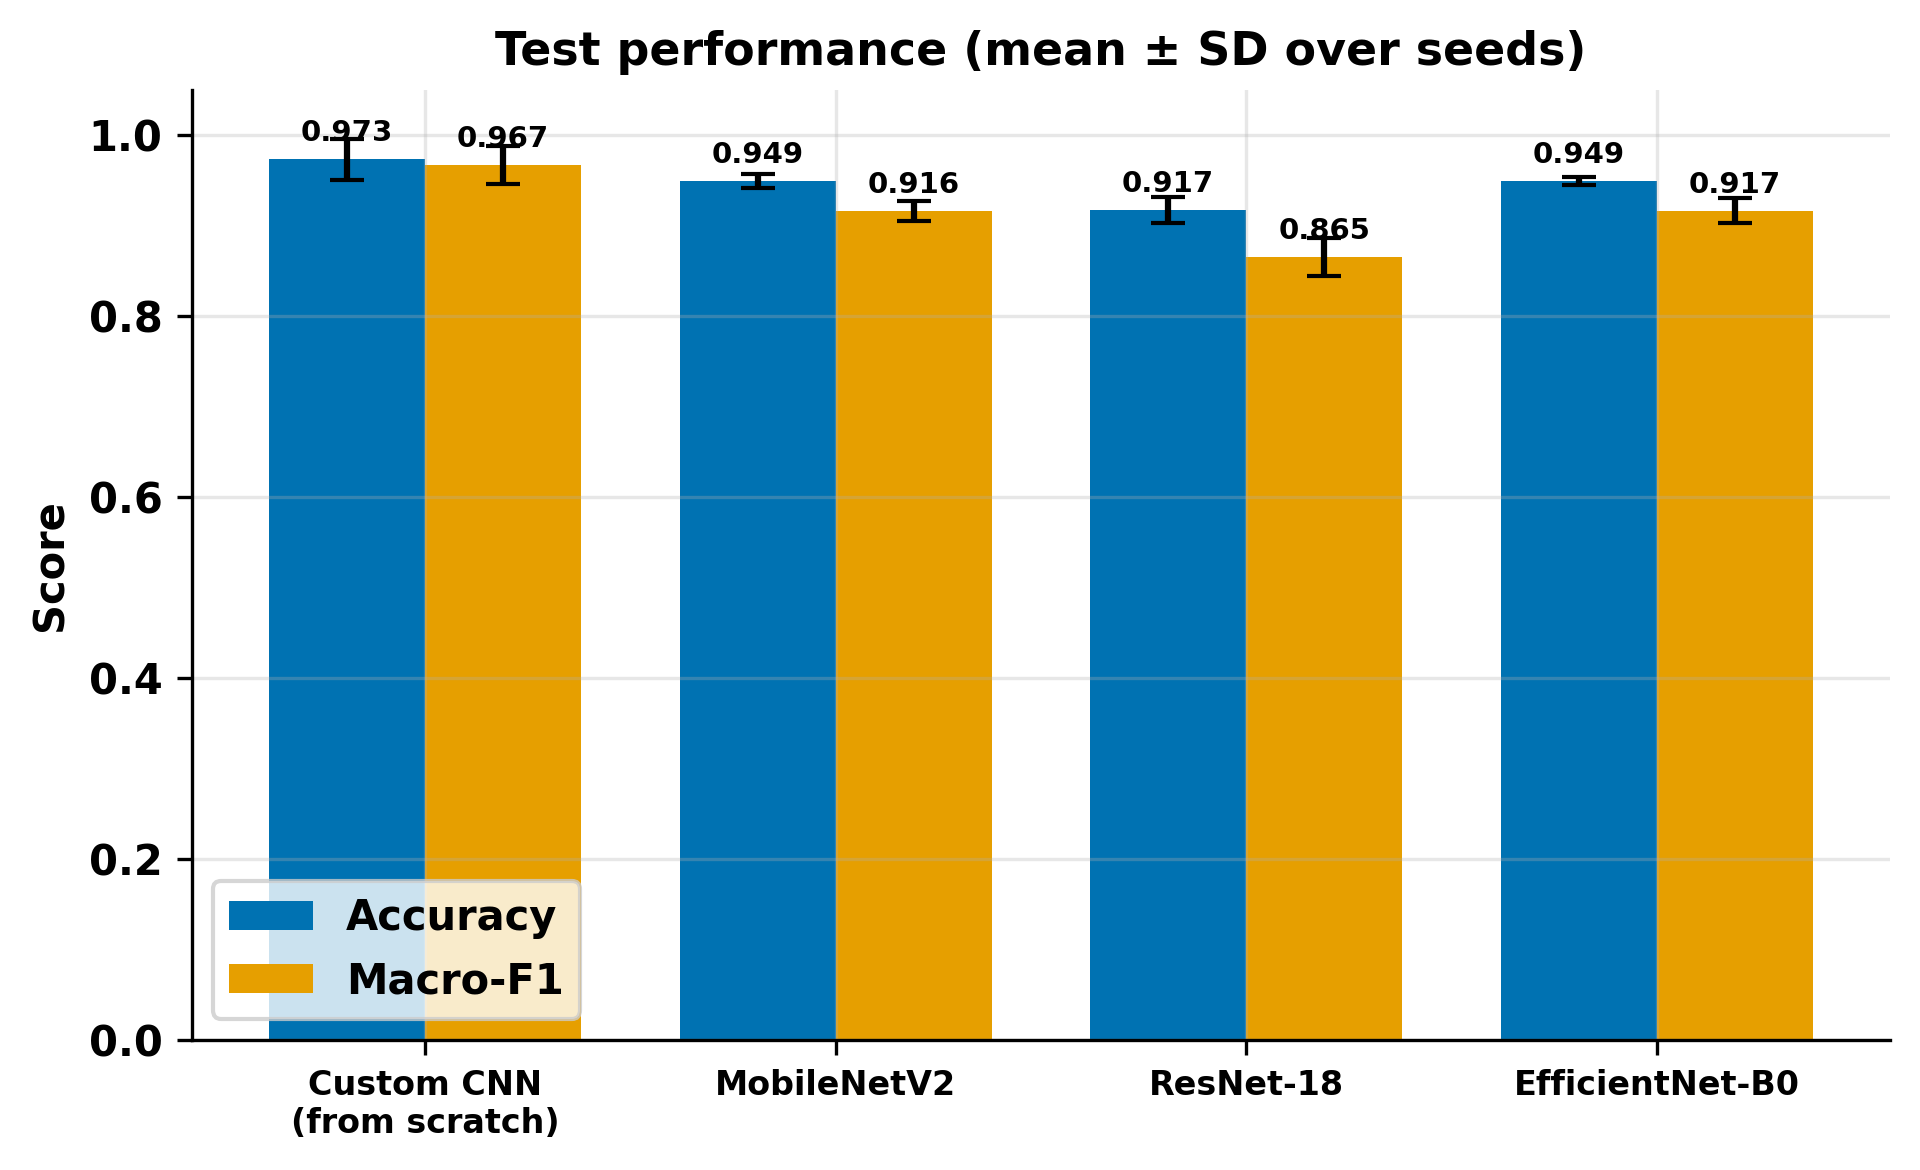
\includegraphics[width=0.7\linewidth]{model_comparison.png}}{\fbox{\parbox{0.6\linewidth}{\centering\vspace{1cm}[model\_comparison.png]\vspace{1cm}}}}
\caption{Exactitud y F1 macro de prueba (media\,$\pm$\,desviación estándar sobre
$\nseeds$ semillas) para los cuatro modelos.}
\label{fig:comparison}
\end{figure}

\begin{figure}[t]
\centering
\IfFileExists{figures/training_curves.png}{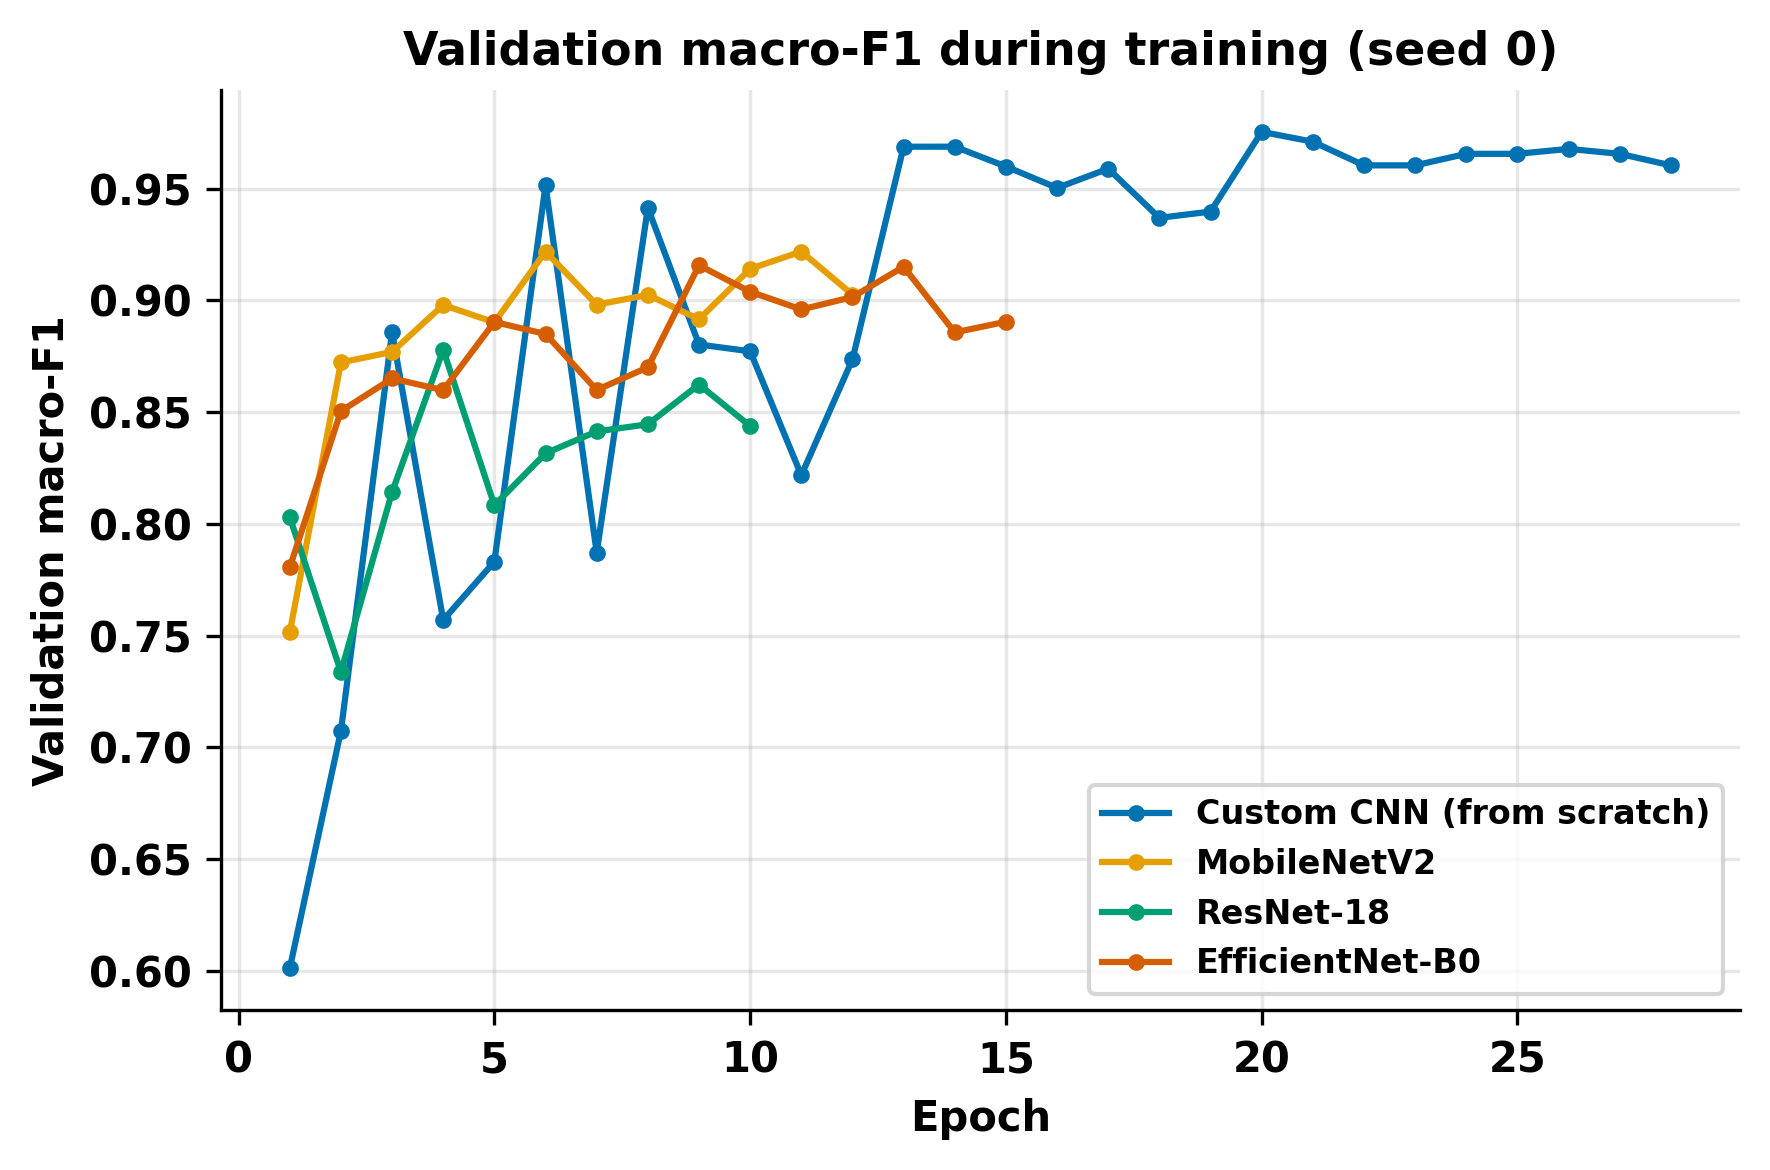
\includegraphics[width=0.62\linewidth]{training_curves.png}}{\fbox{\parbox{0.6\linewidth}{\centering\vspace{1cm}[training\_curves.png]\vspace{1cm}}}}
\caption{F1 macro de validación a lo largo de las épocas de entrenamiento (semilla
representativa). Las redes base preentrenadas convergen rápido; la CNN entrenada desde
cero converge más lentamente a un nivel similar.}
\label{fig:curves}
\end{figure}

\subsection{Estructura de confusión}
Las matrices de confusión (Fig.~\ref{fig:confusion}) son informativas más allá de la
exactitud destacada. Para el mejor modelo (CNN propia) los pocos errores son
predominantemente confusiones enfermedad-versus-enfermedad---un patrón operativamente
benigno, ya que ambos estados enfermos ameritan intervención. Los modelos por
transferencia congelada, más débiles, en cambio clasifican erróneamente además un
número no trivial de hojas con \emph{tizón tardío} como \emph{sanas} (por ejemplo,
10--12 de 150 para MobileNetV2 y ResNet-18): un modo de falso negativo mucho más
preocupante, porque le diría a un agricultor que una planta infectada está sana. Esta
asimetría---el modelo entrenado desde cero no sólo puntúa más alto sino que falla de
forma más segura---refuerza el argumento a favor del modelo compacto de extremo a
extremo. La clase minoritaria sana se reconoce de manera fiable en todos los modelos, lo
que indica que la ponderación de clases contrarresta el desbalance.

\begin{figure}[t]
\centering
\IfFileExists{figures/confusion_matrices.png}{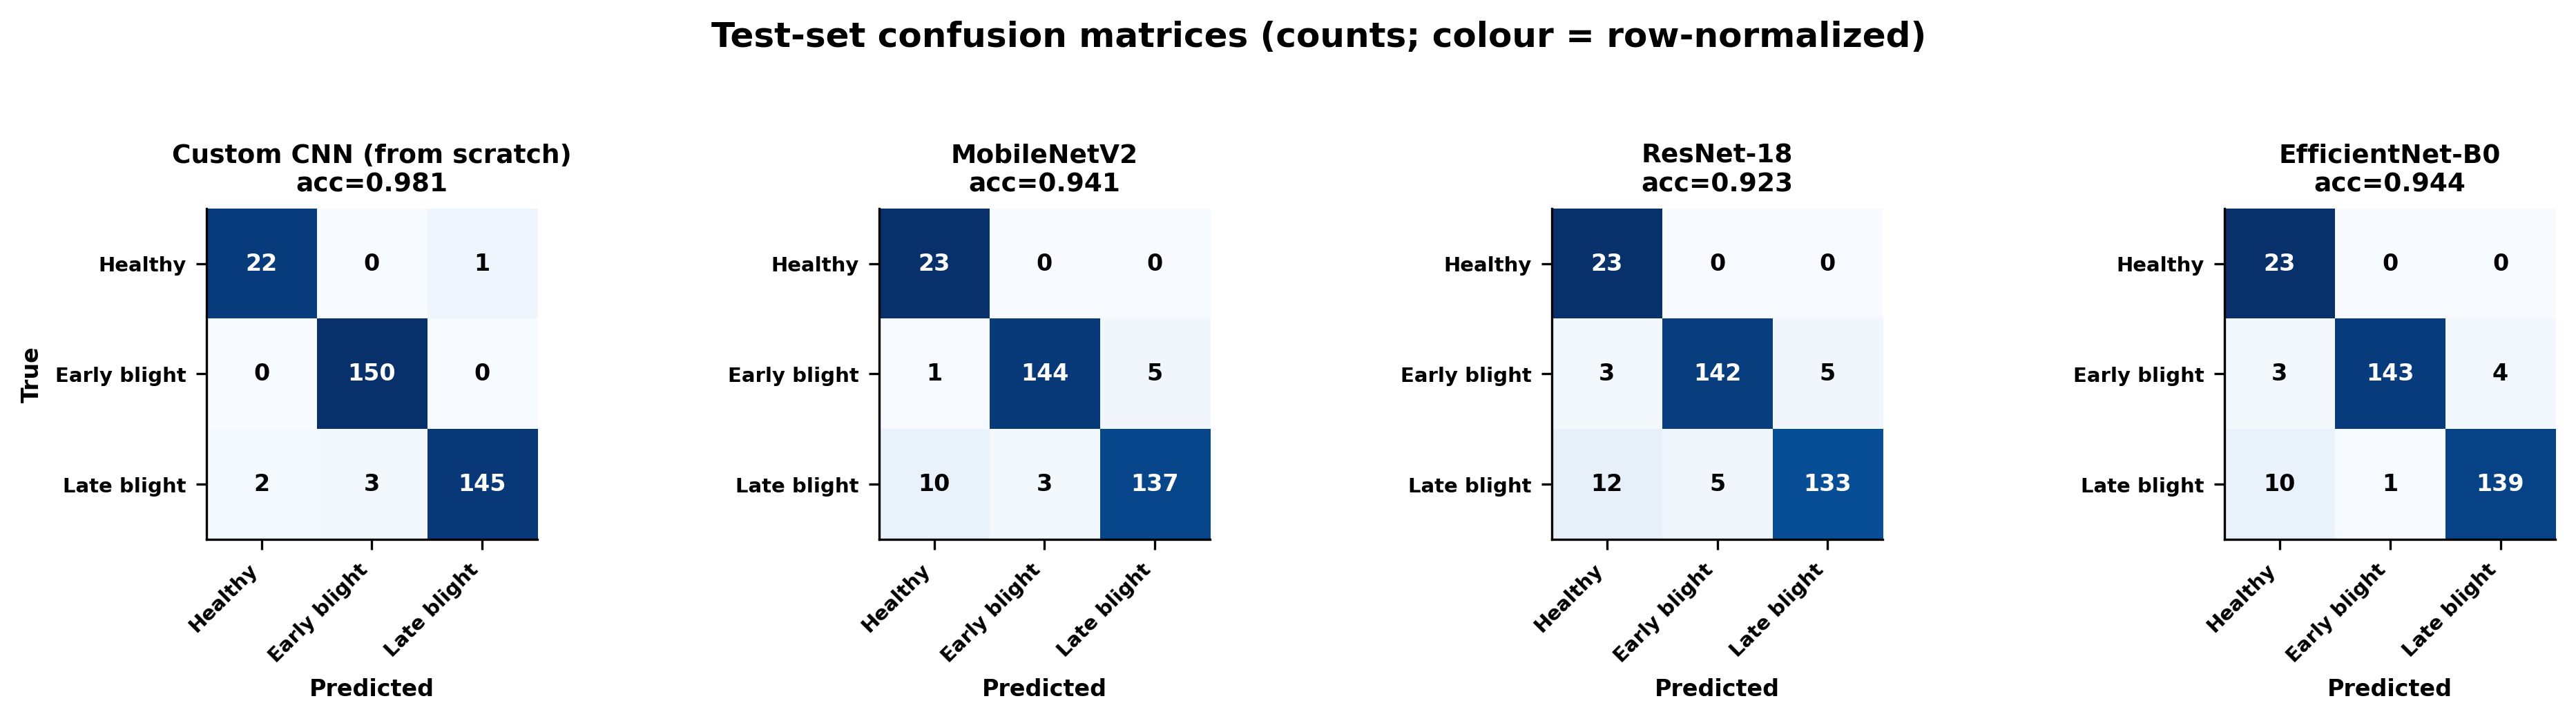
\includegraphics[width=0.98\linewidth]{confusion_matrices.png}}{\fbox{\parbox{0.6\linewidth}{\centering\vspace{1cm}[confusion\_matrices.png]\vspace{1cm}}}}
\caption{Matrices de confusión de prueba por modelo (texto de celda: conteos; color:
tasa normalizada por fila).}
\label{fig:confusion}
\end{figure}

\subsection{Calibración}
Más allá de la exactitud, un diagnóstico desplegable debería reportar confianzas
fiables. La Fig.~\ref{fig:reliability} muestra diagramas de fiabilidad y valores de ECE
(para una semilla representativa; el Cuadro~\ref{tab:results} reporta el ECE promediado
entre semillas). Todos los modelos están imperfectamente calibrados, con un ECE
promediado entre semillas que va de $\eceCustom$ (CNN propia, la mejor calibrada) a
cerca de $0.17$ (ResNet-18). Los diagramas indican que la mala calibración se debe
principalmente a los compartimentos de confianza media, donde la exactitud empírica y
la confianza predicha divergen, más que a un exceso de confianza uniforme. Esta es una
limitación honesta: si bien la CNN propia es a la vez la más exacta y la mejor calibrada
de las cuatro, ninguna está calibrada lo bastante bien como para tomar sus confianzas
crudas al pie de la letra, y un sistema desplegado se beneficiaría de una calibración
posterior (por ejemplo, escalado por temperatura) antes de usar la confianza para
derivar los casos inciertos a un experto humano.

\begin{figure}[t]
\centering
\IfFileExists{figures/reliability_diagrams.png}{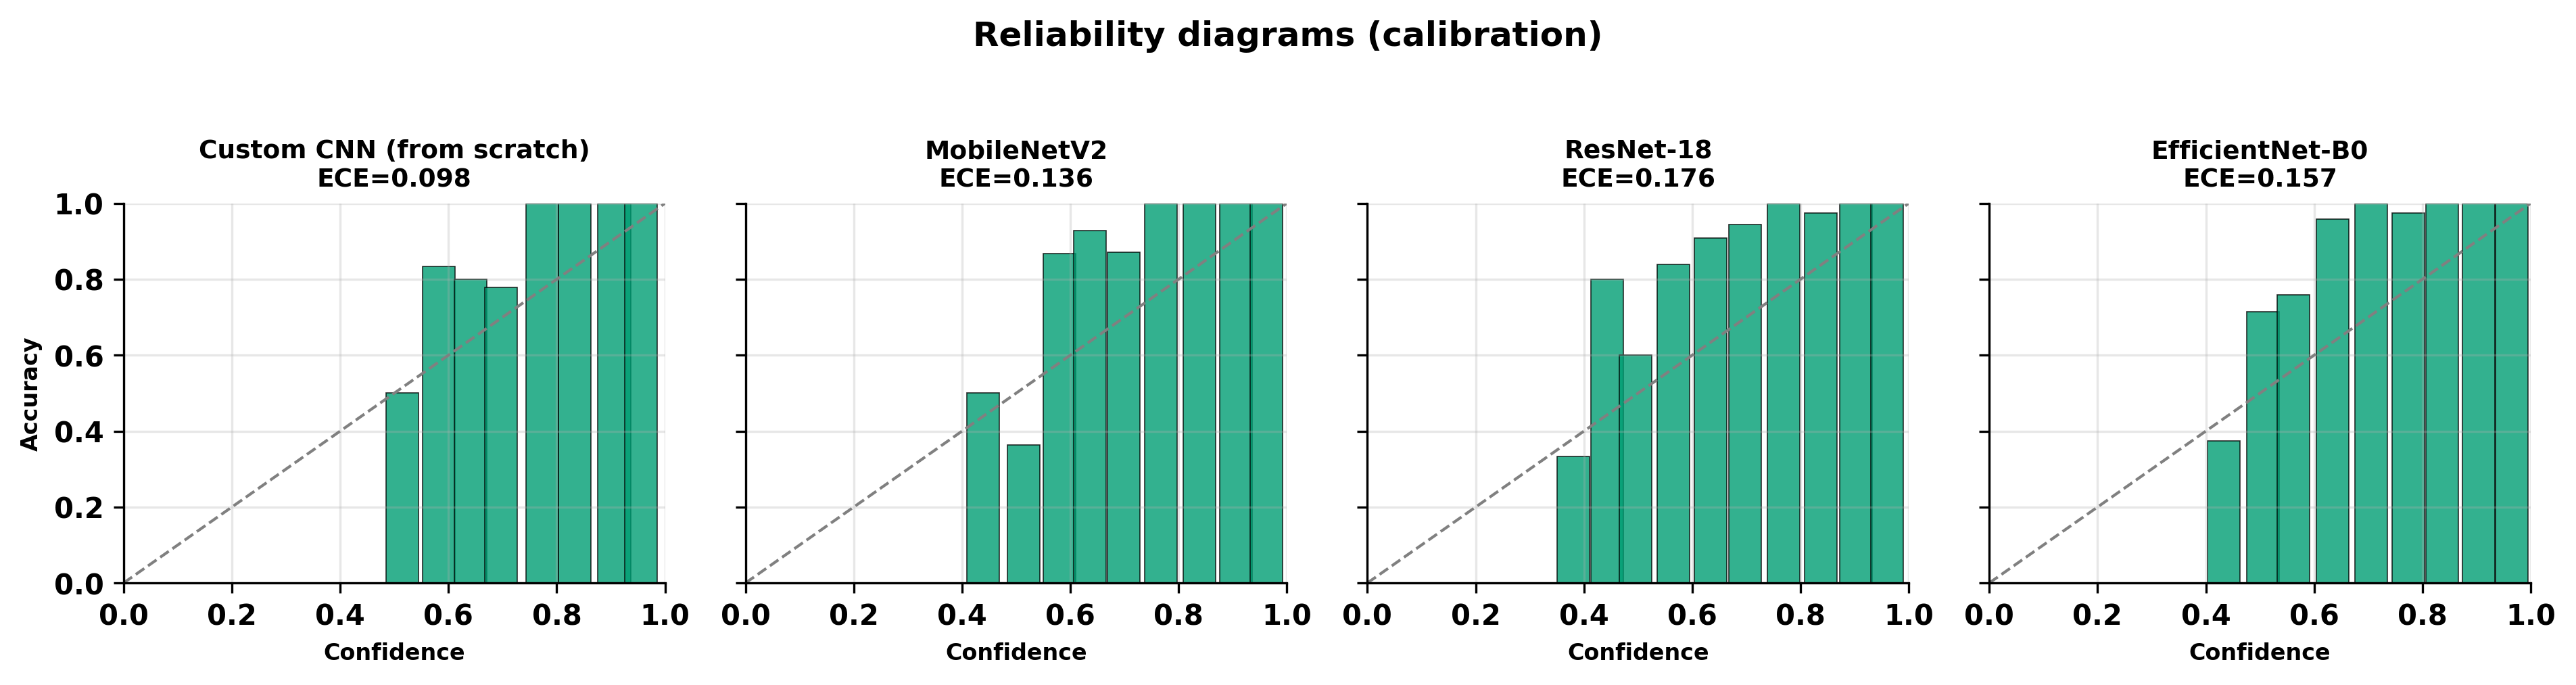
\includegraphics[width=0.98\linewidth]{reliability_diagrams.png}}{\fbox{\parbox{0.6\linewidth}{\centering\vspace{1cm}[reliability\_diagrams.png]\vspace{1cm}}}}
\caption{Diagramas de fiabilidad (calibración). La diagonal punteada es la calibración
perfecta; las barras muestran la exactitud dentro de cada compartimento de confianza.}
\label{fig:reliability}
\end{figure}

\subsection{¿Dónde miran los modelos?}
Los mapas de saliencia de Grad-CAM (Fig.~\ref{fig:gradcam}) aportan la observación
cualitativa más importante del estudio. Aunque los modelos sí ponen atención en las
lesiones visibles para las clases de enfermedad, también asignan una saliencia
sustancial a los bordes de la hoja y al fondo uniforme. Mostramos ejemplos individuales
representativos por clase, de modo que esto es ilustrativo y no una medición
cuantitativa de atribución; no obstante, es visualmente consistente con el sesgo de
fondo que Noyan~\cite{noyan2022uncovering} y Barbedo~\cite{barbedo2018impact}
documentaron, lo que sugiere que parte de la aparente habilidad de los modelos puede
derivar de artefactos del conjunto de datos y no de la patología. A la espera de una
prueba cuantitativa (por ejemplo, ablación del fondo), las exactitudes destacadas se
leen con prudencia como una cota superior del rendimiento real en campo.

\begin{figure}[t]
\centering
\IfFileExists{figures/gradcam_panel.png}{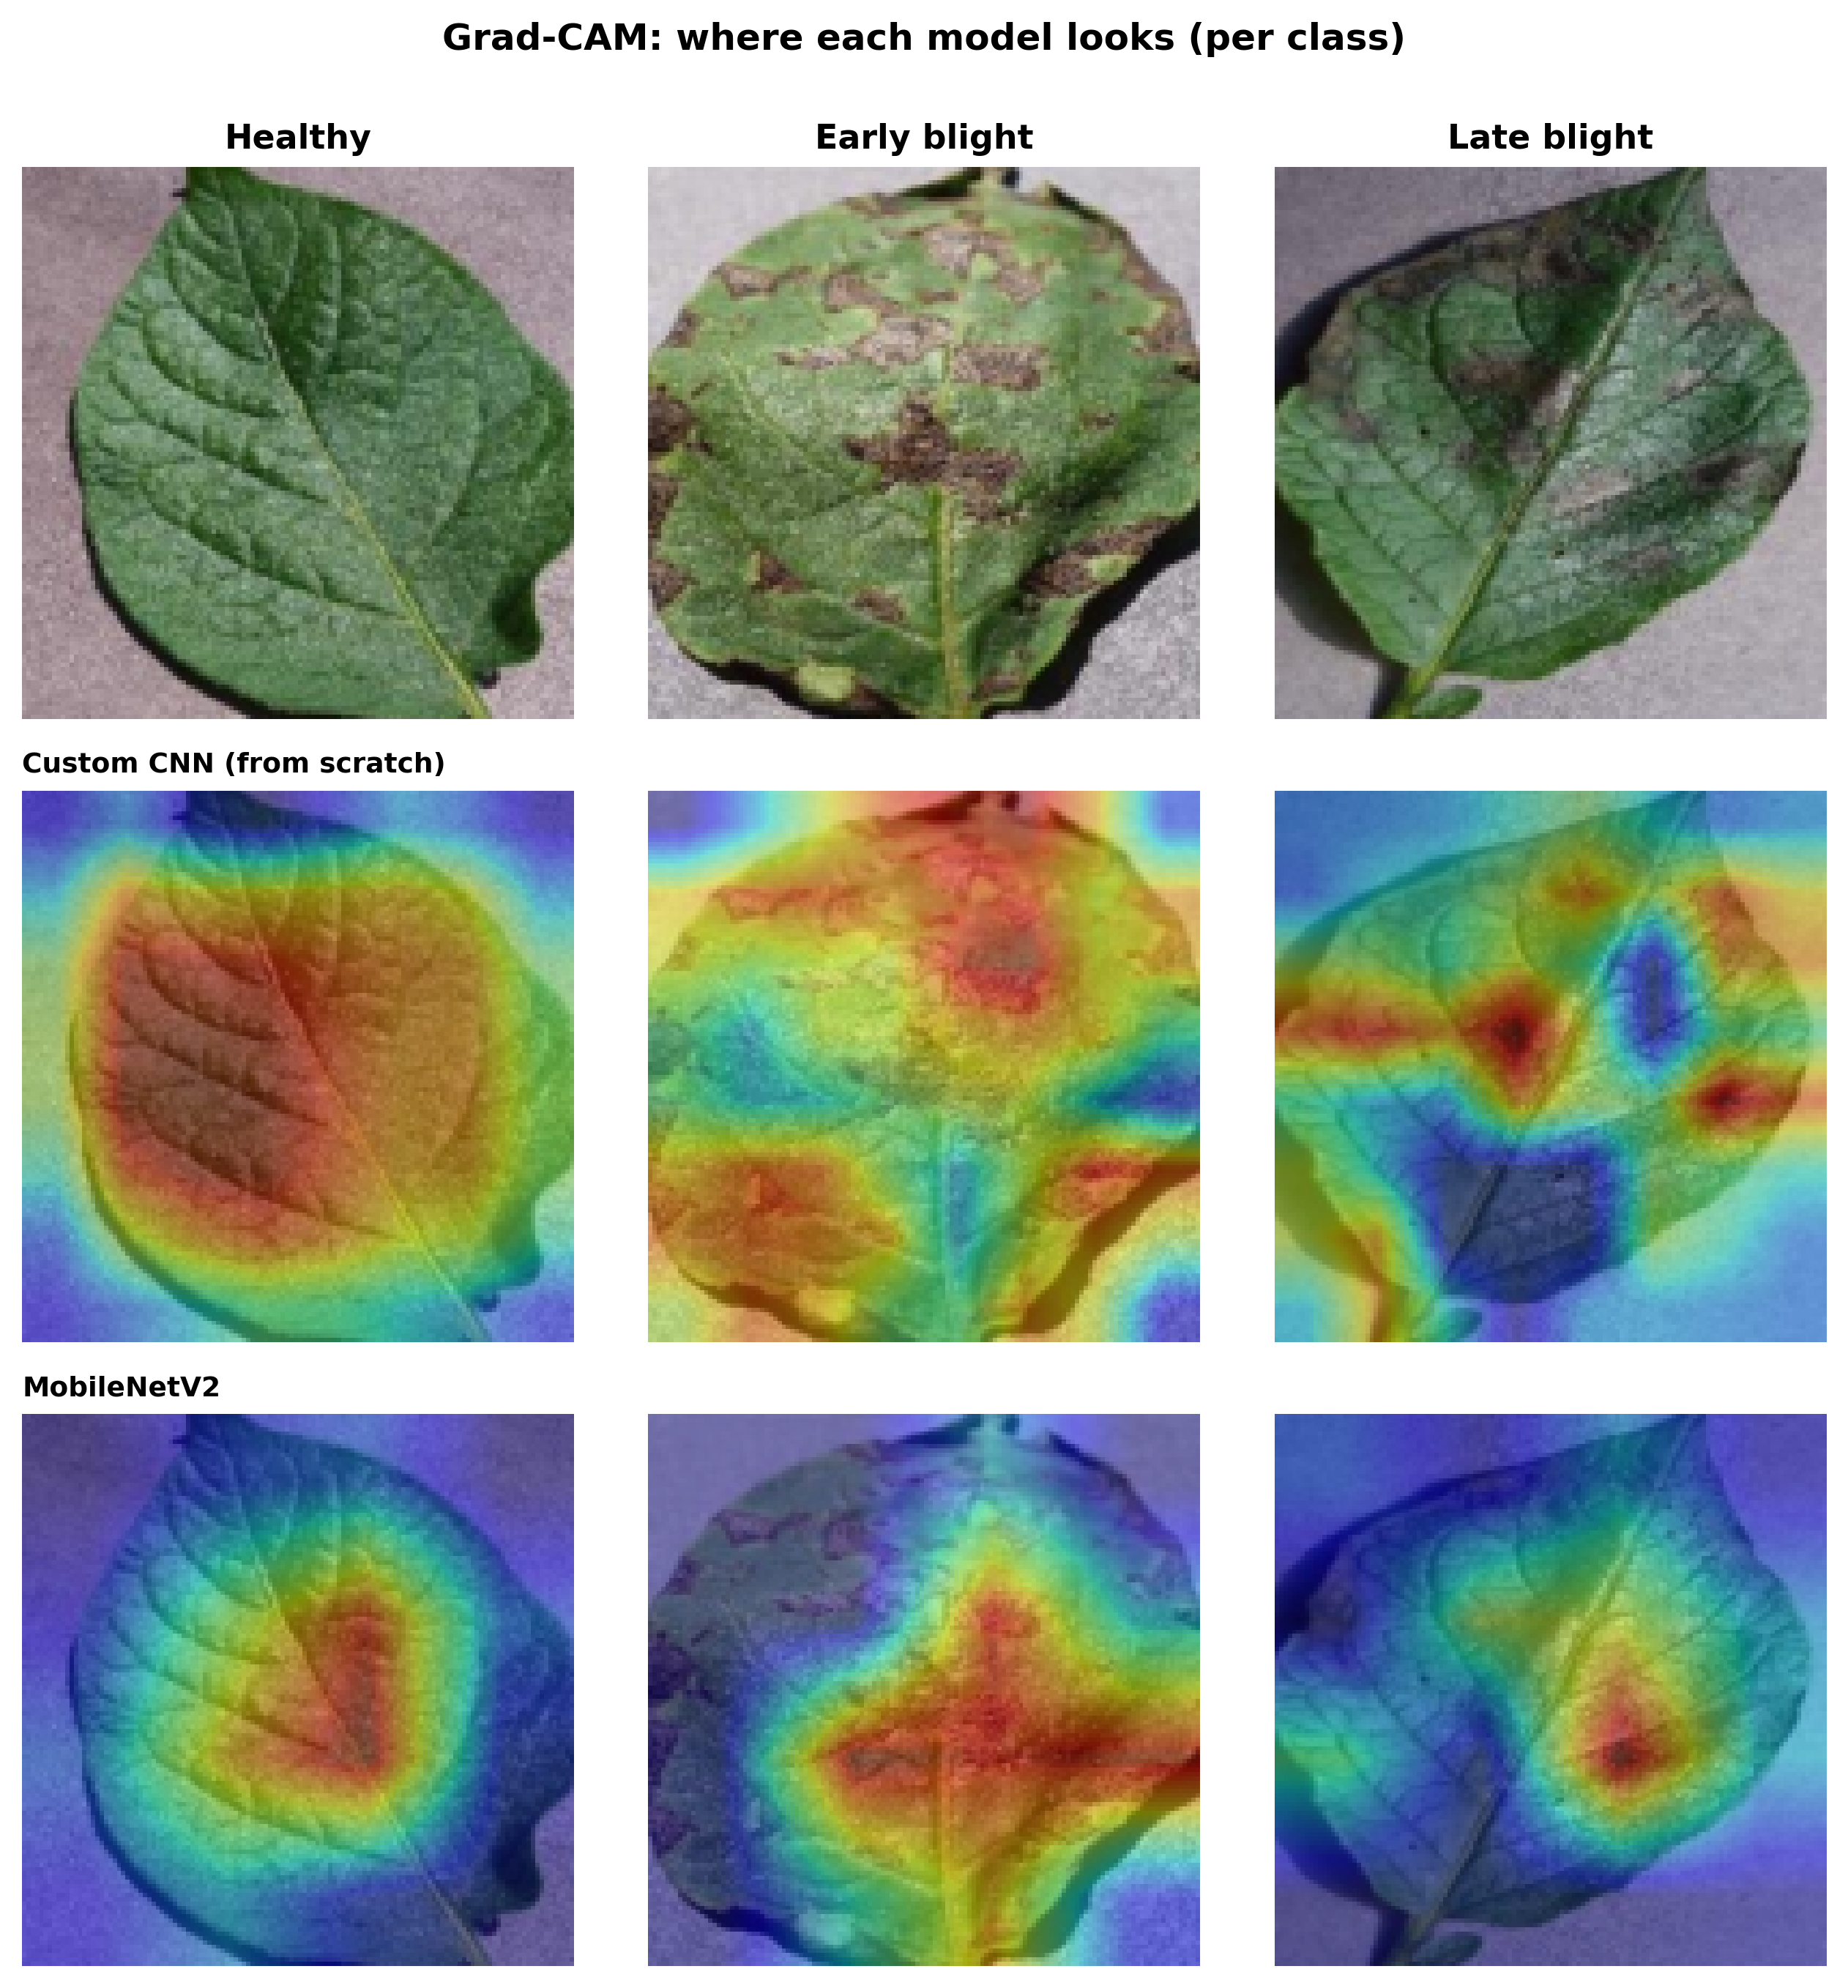
\includegraphics[width=0.95\linewidth]{gradcam_panel.png}}{\fbox{\parbox{0.6\linewidth}{\centering\vspace{1cm}[gradcam\_panel.png]\vspace{1cm}}}}
\caption{Superposiciones de Grad-CAM para un ejemplo representativo por clase. Las
regiones cálidas son las más influyentes para la clase predicha. La atención se
derrama hacia los bordes de la hoja y el fondo, ilustrando una dependencia consistente
con el sesgo de fondo de PlantVillage (cualitativo; no es una métrica cuantitativa de
atribución).}
\label{fig:gradcam}
\end{figure}

\section{Discusión}
Nuestros resultados respaldan una conclusión de dos caras. Por un lado, una CNN pequeña
entrenada desde cero en una laptop \emph{supera}---de forma significativa y
reproducible---a las líneas base de aprendizaje por transferencia de red base congelada
para este problema de tres clases, usando $\paramratiomin$--$\paramratiomax\times$
menos parámetros. Esto debe leerse con cuidado: congelamos las redes base preentrenadas
y entrenamos sólo un cabezal nuevo, la receta estándar de transferencia de bajo
cómputo, de modo que la comparación es específicamente \emph{entrenamiento de extremo a
extremo desde cero frente a transferencia de características congeladas bajo un
presupuesto de cómputo igual y modesto}. Hay también una asimetría que conviene
declarar con claridad: como sus redes base están congeladas, las líneas base actualizan
sólo $\trainheadmin$--$\trainheadmax$ parámetros de cabezal durante el entrenamiento,
mientras que la CNN desde cero optimiza todos sus $\traincustom$ pesos. Por lo tanto,
nuestra ventaja de ``menos parámetros'' se refiere al tamaño \emph{total} del
modelo---lo que debe almacenarse y ejecutarse en inferencia---no al número de pesos
actualizados durante el entrenamiento. Un ajuste fino completo de las redes base muy
probablemente elevaría su exactitud y podría reducir o revertir la brecha, pero también
es sustancialmente más costoso y ávido de datos---precisamente el costo que nos
propusimos evitar. El mensaje práctico se mantiene: para una tarea de diagnóstico
estrecha y bien definida en hardware accesible, un modelo compacto a medida no es un
compromiso sino una opción fuerte y mucho más barata. Por otro lado, el análisis con
Grad-CAM es un resultado de advertencia que ninguna exactitud adicional sobre
PlantVillage puede resolver: como los fondos del conjunto de datos son informativos,
los altos puntajes dentro del conjunto no garantizan robustez en campo.

\textbf{Limitaciones.} El estudio está deliberadamente acotado. Las imágenes de
PlantVillage son capturas de laboratorio con fondos limpios; las imágenes de campo
contienen desorden, iluminación variable y condiciones concurrentes, y esperamos que
todos los modelos se degraden con ellas. La tarea de papa de tres clases es
comparativamente fácil, lo que comprime las diferencias entre arquitecturas. Congelamos
las redes base de transferencia en lugar de ajustarlas por completo, cambiando un poco
de exactitud por velocidad y por una comparación justa de bajo cómputo. No desplegamos
en un dispositivo móvil, aunque los conteos de parámetros sugieren factibilidad.

\textbf{Trabajo futuro.} Los siguientes pasos naturales son la evaluación con imágenes
de papa recolectadas en campo, la eliminación o segmentación explícita del fondo para
forzar al modelo a centrarse en la hoja, y la evaluación en dispositivo de la latencia
y la energía. La canalización reproducible publicada aquí está diseñada para facilitar
esas extensiones.

\section{Conclusión}
Presentamos una comparación reproducible y estadísticamente cuidadosa de una CNN
entrenada desde cero frente a líneas base de aprendizaje por transferencia de red base
congelada para la clasificación de enfermedades en hojas de papa con hardware de
consumo. El modelo compacto a medida---más de un orden de magnitud más pequeño que
ResNet-18 ($\paramratiomax\times$ menos parámetros)---supera significativamente a las
líneas base por transferencia congelada bajo un presupuesto de cómputo igualmente bajo,
y Grad-CAM revela una dependencia compartida del fondo del conjunto de datos que matiza
todas las exactitudes reportadas. El trabajo aboga por un modelado de enfermedades
vegetales honesto, interpretable y accesible en hardware, por encima de la persecución
de tablas de clasificación.

\section*{Contribuciones de autoría}
N.P. concibió y diseñó el estudio, implementó la canalización de datos, los modelos, el
código de entrenamiento y evaluación, ejecutó los experimentos y los análisis
estadísticos, produjo las figuras y redactó y revisó el manuscrito. Al tratarse de un
trabajo de autor único, todas las contribuciones son atribuibles a N.P.

\section*{Disponibilidad de los datos}
El conjunto PlantVillage está disponible públicamente~\cite{hughes2015plantvillage}. El
script de descarga y el subconjunto exacto de papa utilizado se describen en el
repositorio de código; aquí no se redistribuyen datos de imagen.

\section*{Disponibilidad del código}
Todo el código, las configuraciones, las dependencias fijadas y los scripts para
reproducir cada número y figura de este manuscrito están disponibles en
\url{https://github.com/nielspac177/papa-vision}.

\section*{Intereses en competencia}
El autor declara no tener intereses en competencia.

\bibliographystyle{unsrt}
\bibliography{references}

\end{document}
